\chapter{Soluzioni di Kerr-Newman}
Nel capitolo \S\ref{para.schwarz} è stata vista la soluzione di Schwarzschild come prima, sia storicamente sia didatticamente, soluzione alle equazioni di campo di Einstein. In particolar modo la soluzione di Schwarzschild risulta l'unica soluzione che emerge dalle equazioni nel vuoto a simmetria sferica, come enunciato dal teorema di Birkhoff\footnote{Se è presente della carica, quindi si è in un sistema di equazioni di Einstein-Maxwell come fatto fra poco, allora la soluzione di Reissner-Nordstr\"om è l'unica sfericamente simmetrica.}.

Ulteriori soluzioni esatte alle equazioni di Einstein sono possibili e rientrano nella più generale metrica di Kerr-Newman. Per fare ciò sarà necessario alleggerire la richiesta di simmetria sferica, che come visto portava alla sola soluzione di Schwarzschild, per favorire l'assisimmetria. Il motivo per cui le soluzioni esatte siano trovate in spazi ad alta simmetria, è ovviamente dovuto alla complessità delle equazioni di Einstein.
Esistono teoremi di unicità per le soluzioni assisimmetriche, oltre a quello di Birkhoff.

\begin{definizione}
Uno spaziotempo asintoticamente piatto è \textbf{assisimmetrico} se esiste un campo vettoriale di Killing $m$ di tipo spazio vicino all'infinito spaziale e per cui tutte le orbite sono chiuse.

Si possono scegliere delle coordinate tali che $m = \partial_\phi$ è una coordinata di modulo $2\pi$.
\end{definizione}
\begin{teorema}[di Carter-Robinson]
Se $(\mathcal{M},g)$ è uno spaziotempo asintoticamente piatto, stazionario e assisimmetrico con $R_{\mu\nu} =0$ , non singolare fuori e sopra l'orizzonte, allora $(\mathcal{M}, g)$  è membro della famiglia di Kerr a due parametri $m$ (massa) e $J$ (momento angolare).
\end{teorema}

Questo teorema ci assicura l'esistenza della soluzione di Kerr.
La richiesta che lo spaziotempo sia assisimmetrico non è del tutto necessaria in quanto, per i buchi neri la stazionarietà implica l'assisimmetria.

Il teorema può essere ulteriormente generalizzato se si considera un sistema di equazioni di Einstein- Maxwell, quindi soddisfacenti l'azione eq. \ref{eq.azione_einstein_maxwell} che produce le equazioni del moto eq. \ref{eq.equazioni_einstein_maxwell}. 
In tal caso i buchi neri asintoticamente piatti e stazionari devono appartenere alla famiglia di Kerr-Newman a 3 parametri\footnote{Questo teorema viene chiamato \textit{no-hair theorem}. Jacob Bekenstein coniò questo nome dicendo che \virgolette{black holes have no hair} per esprimere un caratteristica dei buchi neri tutt'altro che banale:  tutte le proprietà che possiede la materia che componeva stelle collassate in buchi neri (campi magnetici, correnti di materia, rotazioni differenziali, inomogeneità) o particelle che accrescono quelli già esistenti (spin, numero leptonico o barionico) scompaiono una volta attraversato l'orizzonte degli eventi, nel senso che diventano permanentemente inaccessibili agli osservatori all'esterno, i quali riescono a descrivere il buco nero con solo questi tre parametri. Wheeler riportò in un'intervista che secondo Feynman la frase usata da Bekenstein fosse oscena e non volesse usarla.} (o 4 se consideriamo le cariche separate):
\begin{align}
    ds^2 &= - \frac{\Delta - a^2\sin^2\theta}{\rho^2}dt^2 - 2a\sin^2\theta\frac{r^2+a^2- \Delta}{\rho^2}dtd\phi + \nonumber \\
    & + \frac{(r^2+a^2)^2 - \Delta a^2\sin^2\theta}{\rho^2}\sin^2\theta d\phi^2 + \frac{\rho^2}{\Delta}dr^2 + \rho^2 d\theta^2
    \label{eq.metrica_kerr_newman}
\end{align}
dove:
\begin{align*}
    \rho^2 &= r^2 +a^2\cos^2\theta \\
    \Delta &= r^2 -2mr + a^2 + e^2
\end{align*}
metrica  che è accoppiata alla Maxwell 1-forma:
\begin{equation}
    A^2 = \frac{1}{\rho^2}\left[Qr(dt - a\sin^2\theta d\phi) - P\cos\theta[ adt - (r^2+a^2)d\phi] \right]
    \label{eq.maxwell_1forma}
\end{equation}
I parametri $a$, $m$ sono rispettivamente parametri di rotazione e massa, mentre $Q$, $P$ sono carica elettrica e magnetica che definiscono il terzo parametro:
\begin{equation*}
    e^2 = Q^2 + P^2
\end{equation*}
Può essere mostrato che il parametro di rotazione è collegato al momento angolare totale $J$ secondo:
\begin{equation*}
    a = \frac{J}{m}
\end{equation*}
Il sistema di coordinate $(t,r,\phi,\theta)$ che descrive la metrica eq. \ref{eq.metrica_kerr_newman} è chiamato di \textbf{Boyer-Lindquist}.

Si possono notare i seguenti casi limite:
\begin{itemize}
    \item $a = e = 0$ è la soluzione di Schwarzschild (non rotante, non carico, sfericamente simmetrico, statico).
    \item $a = 0$ è la soluzione di Reissner-Nordstr\"om (non rotante, carico, sfericamente simmetrico, statico).
    \item $e=0$ è la soluzione di Kerr (rotante, non carico, assisimmetrico, stazionario).
\end{itemize}
\section{Soluzione di Reissner-Nordstr\"om}
Questa soluzione permette di descrivere lo spazio esterno ad un corpo a simmetria sferica, carico e permette di generalizzare la soluzione di Schwarzschild. La metrica è:
\begin{equation}
    ds^2 = - \left(1 - \frac{2M}{r} + \frac{e^2}{r^2}\right)dt^2 + \frac{dr^2}{1 - \frac{2M}{r} + \frac{e^2}{r^2}} + r^2(d\theta^2 + \sin^2\theta d\phi^2)
    \label{eq.metrica_rn}
\end{equation}
e la Maxwell 1-forma\footnote{Può anche essere letta come $A^\mu = (\frac{Q}{r},0,0,P\cos\theta)$.}:
\begin{equation*}
    A = \frac{Q}{r}dt + P\cos \theta d\phi
\end{equation*}
L'orizzonte è determinato dalla singolarità delle coordinate, corrispondente ai valori:
\begin{equation*}
  r_{\pm} = M \pm \sqrt{M^2 - e^2}  
\end{equation*}
dove $r_+$ è detto orizzonte degli eventi, mentre $r_-$ è l'orizzonte di Cauchy. 
Poiché questi valori possono essere complessi, si ha un limite superiore alle cariche affinché possa essere ottenuto un buco nero:
\begin{equation*}
    P^2 + Q^2 \leq M^2
\end{equation*}
Per $e^2 > M^2$ non ci sono orizzonti e la singolarità è nuda. Il caso $r_+ = r_-$ è detto buco nero estremale.

\subsection{Buco nero estremale, soluzione di Bertotti-Robinson e di Majumdar-Papapetrou}
La metrica eq. \ref{eq.metrica_rn} diventa per $M=e$:
\begin{equation*}
    ds^2 = - \left(1 - \frac{e}{r} \right)^2dt^2 + \left(1 - \frac{e}{r} \right)^{-2}dr^2 + r^2 d\Omega^2
\end{equation*}
Introducendo la coordinata radiale:
\begin{equation*}
    \rho = r - e
\end{equation*}
detta \textbf{coordinata isotropa}, l'orizzonte viene portato al valore $\rho = 0$. Dunque la metrica diventa:
\begin{equation}
    ds^2 = - \left( 1 + \frac{e}{\rho}\right)^{-2}dt^2 +  \left( 1 + \frac{e}{\rho}\right)^2\left[ d\rho^2 + \rho^2 d\Omega^2\right]
    \label{eq.metrica_rn_estremale_isot}
\end{equation}
Si può far notare che la funzione $1 + \frac{e}{\rho}$ sia una funzione armonica di $\mathbb{E}^3$.
Studiamo la geometria vicino all'orizzonte: approssimiamo per $\rho \rightarrow 0$, $1 + \frac{e}{\rho} \simeq \frac{e}{\rho}$ così:
\begin{equation*}
    ds^2 = - \frac{\rho^2}{e^2}dt^2 + \frac{e^2}{\rho^2}d\rho^2 + e^2 d\Omega^2
\end{equation*}
In questa metrica si può riconoscere che la geometria è lo spazio prodotto $AdS_2 \times S^2$ , dove Anti-de Sitter è scritto in coordinate di Poincarè, mentre la 2-sfera ha raggio pari a $e$. Questa soluzione vicino all'orizzonte è detta \textbf{di Bertotti-Robinson}. Il gruppo di isometrie vicino all'orizzonte viene allargato da $\mathbb{R}\times SO(3)$ a $O(2,1)\times SO(3)$.

\'E possibile generalizzare la metrica e il potenziale di gauge $A$ a:
\begin{equation*}
        ds^2 = - V(\bm{x})^{-2}dt^2 + V(\bm{x})^2 d\bm{x}^2
\end{equation*}
\begin{equation*}
        A = V(\bm{x})^{-1}dt
\end{equation*}
dove, affinché siano soddisfatte le equazioni di Einstein:
\begin{equation*}
    \nabla^2_{\mathbb{E}^3} V(\bm{x}) = 0
\end{equation*}
Questa viene detta \textbf{soluzione di Majumdar-Papapetrou}.

Un caso particolare è dato dalla funzione armonica:
\begin{equation*}
    V(\bm{x}) = 1 + \sum_{i=1}^N \frac{M_i}{|\bm{x} - \bm{x}_i|}
\end{equation*}
corrispondente ad una configurazione di $N$ buchi neri di massa $M_i$ posti in $\bm{x}_i$.
Questo rappresenta un principio di sovrapposizione nella relatività generale che, data la natura fortemente non lineare delle equazioni di Einstein, non è fatto per nulla scontato. Ciò è possibile perché vi è un esatto bilancio tra le forze di attrazione gravitazionale con la repulsione elettrostatica. Dunque è solo possibile nel caso estremale.

\section{Soluzione di Kerr}
A differenza della soluzione di Schwarzschild, scoperta poco dopo la pubblicazione della relatività generale e la sua estensione carica con la metrica di Reissner-Nordstr\"om, ricavata sempre in quegli anni, ci sono voluti una cinquantina di anni per ottenere, nel 1963 grazie a R. Kerr, una metrica che descrivesse lo spaziotempo generato da un corpo non carico e rotante.
Ad oggi la metrica viene ricavata dalla più generale famiglia di Kerr-Newman, eq. \ref{eq.metrica_kerr_newman}, imponendo $e = 0$:
\begin{align}
ds^2 &= - \frac{\Delta - a^2\sin^2\theta}{\rho^2}dt^2 - 2a\sin^2\theta\frac{2mr}{\rho^2}dtd\phi + \nonumber \\
&+ \frac{(r^2 + a^2)^2- \Delta a^2\sin^2\theta}{\rho^2}\sin^2\theta d\phi^2 + \frac{\rho^2}{\Delta}dr^2 + \rho^2 d\theta^2
    \label{eq.metrica_kerr}
\end{align}
dove $\Delta = r^2 -2mr + a^2$ e $\rho^2 = r^2 + a^2\cos^2\theta$. Questa metrica è particolarmente importante dal punto di vista astrofisico, in quanto permette di descrivere le stelle rotanti a grandi distanze e i buchi neri astrofisici, che si osservano non possedere carica.  Il termine $g_{tt}$ può essere anche scritto nella forma:
\begin{equation*}
    g_{tt}= -\left( 1 - \frac{2M}{\rho^2}\right)
\end{equation*}
La soluzione di Kerr è una soluzione esatta alle equazioni di Einstein per $r > R$, con $R$ il raggio del corpo; non è stata accoppiata a nessuna soluzione che rappresenti l'interno di una stella, a differenza di Schwarzschild che, grazie al teorema di Birkhoff, descrive lo spaziotempo esterno esatto che si accoppia ad una soluzione interna sfericamente simmetrica\footnote{In \cite{tong} viene fatto notare che i teoremi di unicità come Carter-Robinson fanno uso esplicito dell'orizzonte degli eventi, mentre per Birkhoff l'unica assunzione è la simmetria sferica. Questo causa quanto appena detto. Inoltre rende la soluzione di Kerr valida come approssimazione a grandi distanze dalla superficie della stella.} .

La metrica di Kerr nel limite $M\rightarrow 0$ con $a$ fissato, si riduce alla metrica di Minkowski. Infatti ha la forma:
\begin{equation*}
    ds^2 = -dt^2 + \frac{r^2 + a^2\cos^2\theta}{r^2 + a^2}dr^2 + (r^2+a^2)\sin^2\theta d\phi^2 + (r^2 + a^2\cos^2\theta)d\theta^2
\end{equation*}
che con la trasformazione di coordinate:
\begin{equation*}
    \left\{ \begin{array}{l}
        \rho = \sqrt{r^2 + a^2}\sin\theta \\
        z = r\cos\theta          
    \end{array}\right.
\end{equation*}
i riduce a Minkowski in coordinate cilindriche, $ds^2 = -dt^2 + d\rho^2 +\rho^2 d\phi^2 + dz^2$.

La metrica di Kerr presenta due isometrie continue con i vettori di Killing che in opportune coordinate possono essere scritti (attenzione a non confondere il vettore di Killing $m$ con la massa):
\begin{equation*}
    k = \partial_t \qquad m =\partial_\phi
\end{equation*}
Kerr nella forma di Boyer-Lindquist, presenta una singolarità delle coordinate per $\Delta = (r - r_-)(r-r_+) = 0$ dove:
\begin{equation*}
    r_\pm = m \pm \sqrt{ m^2 - a^2}
\end{equation*}
Questa metrica è invariante sotto inversione simultanea di $t$ e $\phi$, mentre non lo è per la sola inversione temporale (a meno che $a=0$, ma è Schwarzschild): infatti l'inversione del tempo di un oggetto rotante determina l'oggetto in rotazione nel senso opposto.

Si distinguono 3 casi:

\subsubsection{$m^2 < a^2$} 
In questo caso $r_\pm \in \mathbb{C}$ e pertanto non c'è alcuna singolarità delle coordinate, solo quella di curvatura in $\rho = 0$ che corrisponde a $r= 0$ all'equatore $\theta = \frac{\pi}{2}$. Si verifica che è proprio di curvatura calcolando uno scalare di curvatura, come ad esempio $R_{\mu\nu\rho\sigma}R^{\mu\nu\rho\sigma}$.

La natura di questa singolarità può essere studiata nelle \textbf{coordinate di Kerr-Schild} definite secondo:
\begin{align*}
    x + iy &= (r + ia)\sin\theta e^{i \int ( d\phi + \frac{a}{\Delta}dr)} \\
    z &= r\cos\theta \\
    \Tilde{t} &= \int ( dt + \frac{r^2 + a^2}{\Delta}dr) -r
\end{align*}
che implica che  $r = r(x,y,z)$ sia dato implicitamente da:
\begin{equation*}
    r^4 - (x^2 + y^2 + z^2 - a^2)r^2 - a^2z^2 = 0
\end{equation*}
La metrica in queste coordinate è:
\begin{align}
    ds^2 &= - d\Tilde{t}^2 + dx^2 + dy^2 + dz^2 + \nonumber \\
 &+\frac{2mr^3}{r^4+a^2z^2}\left[ \frac{r(xdx + ydy) - a(xdy -ydx)}{r^2 + a^2} + \frac{zdz}{r} + d\Tilde{t}\right]^2
\label{eq.metrica_kerr_schild}
\end{align}
Si può notare che lo spaziotempo è piatto di Minkowski quando $m=0$.  Infatti per le coordinate di Kerr-Schild vale sempre la scrittura\footnote{Esistono anche i \textit{double Kerr-Schild} per i quali vale $g_{\mu\nu} = \eta_{\mu\nu} + k_\mu k_\nu + l_\mu l_\nu$}:
\begin{equation}
    g_{\mu\nu} = \eta_{\mu\nu} + k_\mu k_\nu
\end{equation}

Si può osservare che le superfici $r=\textrm{cost.}$, $\Tilde{t}= \textrm{cost.}$ sono ellissoidi confocali che degenerano in $r= 0$ al disco:
\begin{align*}
    z = 0 && x^2 + y^2 \leq a^2
\end{align*}
ovvero:
\begin{equation*}
    (x+iy)(x-iy) = (r^2 + a^2)\sin^2\theta \leq r^2 + a^2
\end{equation*}
La singolarità di curvatura ottenuta a $\theta = \frac{\pi}{2}$ corrisponde al bordo del disco $z = 0$, $x^2 +y^2 = a^2$ e viene detta \textbf{ring singularity}.

Inoltre, a differenza di Schwarzschild, non c'è motivo di restringere $r$ ai soli valori positivi, pertanto lo spaziotempo può essere continuato analiticamente attraverso il disco ad un'altra regione asintoticamente piatta dove però $r < 0$.

Possiamo inoltre mostrare la struttura causale di questa soluzione. Poiché Kerr gode di simmetria assiale e non sferica, sarebbe necessario un diagramma 3d per le coordinate $(t,r,\theta)$; tuttavia possiamo restringerci alle sottovarietà $\theta = 0$ e $\theta = \frac{\pi}{2}$ in quanto queste sono \textbf{totalgeodetiche}, ovvero le geodetiche delle sottovarietà lo sono per la varietà stessa o in altre parole le geodetiche inizialmente tangenti alla sottovarietà, rimangono tangenti alla sottovarietà.
In fig. \ref{fig.kerr_causale_1}
\begin{figure}
    \centering
    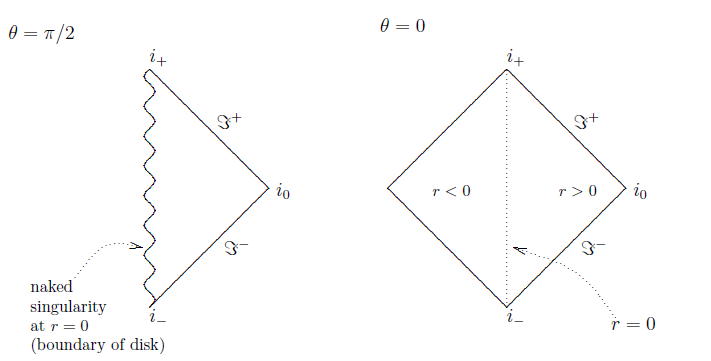
\includegraphics[scale=0.7]{immagini/kerr_causale_1.png}
    \caption{Struttura causale per Kerr con $m^2 < a^2$ per la sottovarietà equatoriale $\theta = \frac{\pi}{2}$ e per lungo l'asse $\theta = 0$. Nel primo caso, la geodetica nulla radiale e ingoing colpisce la ring singularity a $r=0$: la singolarità è nuda. Nel secondo caso le stesse geodetiche lungo l'asse di simmetria attraversano il disco in $r=0$ e finiscono in $r<0$.}
    \label{fig.kerr_causale_1}
\end{figure}
Il motivo principale per cui questo spaziotempo non è fisico è dovuto al vettore di Killing $\partial_\phi$ che diventa di tipo tempo in $r<0$, vicino alla ring singularity. Ciò determina un comportamento non causale in quanto le orbite di $\partial_\phi$ sono chiuse. Nel dettaglio:
\begin{equation*}
    \partial^2_\phi = g_{\phi\phi} = a^2\sin^2\theta \left( 1 + \frac{r^2}{a^2}\right) + \frac{ma^2}{r}\left( \frac{2\sin^4\theta}{1 + \frac{a^2}{r^2}\cos^2\theta}\right) 
\end{equation*}
Quando $r/a = \delta \ll 1$ e considerando $\theta = \pi/2 + \delta$ si ha allora:
\begin{equation*}
    \partial^2_\phi = a^2 + \frac{Ma}{\delta} + o(\delta) < 0
\end{equation*}
quando $\delta$ è sufficientemente piccolo e negativo (vicino $r<0$).
\subsubsection{$m^2 > a^2$}
In questo caso c'è una ring singularity, ma la metrica ha singolarità delle coordinate in $r_\pm$ con Boyer-Lindquist. Per questo motivo si introducono le \textbf{coordinate di Kerr}:
\begin{align*}
    dv &= dt + \frac{r^2 + a^2}{\Delta} dr\\
    d\chi &= d\phi + \frac{a}{\Delta}dr
\end{align*}
e la metrica diventa:
\begin{align}
    ds^2 &= - \frac{\Delta - a^2\sin^2\theta}{\rho^2}dv^2 + 2dvdr - \frac{2a\sin^2\theta(r^2 + a^2 - \Delta)}{\rho^2}dvd\chi + \nonumber \\ &- 2a\sin^2\theta d\chi dr + \frac{(r^2 + a^2)^2 - \Delta a^2\sin^2\theta}{\rho^2}\sin^2\theta d\chi^2 + \rho^2 d\theta^2
\label{eq.metrica_kerr_coord_kerr}
\end{align}

Si può mostrare che le ipersuperfici $r = r_\pm$ sono orizzonti di Killing per i vettori di Killing:
\begin{equation*}
    \xi_\pm = \partial_t + \frac{a}{r^2_\pm + a^2} \partial_\phi
\end{equation*}
E la rispettiva gravità superficiale è:
\begin{equation}
    \kappa_\pm =\frac{r_\pm - r_\mp}{2(r^2_\pm + a^2)}
\label{eq.grav_sup_kerr}
\end{equation}
La struttura causale è mostrata in fig. \ref{fig.kerr_causale_2}.
L'orizzonte degli eventi è a sua volta un orizzonte di Killing di:
\begin{equation*}
    \xi = \partial_t + \Omega_H \partial_\phi
\end{equation*}
con
\begin{equation}
    \Omega_H = \frac{a}{r^2_+ + a^2}
    \label{eq.omega_kerr}
\end{equation}
Segue che se applichiamo $\xi$ a $\phi - \Omega_H t$,:
\begin{equation*}
    \xi(\phi - \Omega_H t) = (\partial_t + \Omega_H \partial_\phi) (\phi - \Omega_H t) = - \Omega_H + \Omega_H = 0
\end{equation*}
Pertanto $\phi = \Omega_H t + \textrm{cost.}$ sulle orbite di $\xi$; allo stesso tempo $\phi = \textrm{cost.}$ sulle orbite di $\partial_t$. Queste informazioni ci permettono di affermare che le particelle su orbite di $\xi$ ruotano con velocità angolare $\Omega_H$ relativa a quelle statiche, su orbite di $\partial_t$, e quindi rispetto un sistema di riferimento stazionario posto all'infinito.
I generatori nulli dell'orizzonte seguono orbite di $\xi$ e ciò ci fa dire che il buco nero di Kerr ruota con velocità angolare $\Omega_H$.
\begin{figure}
    \centering
    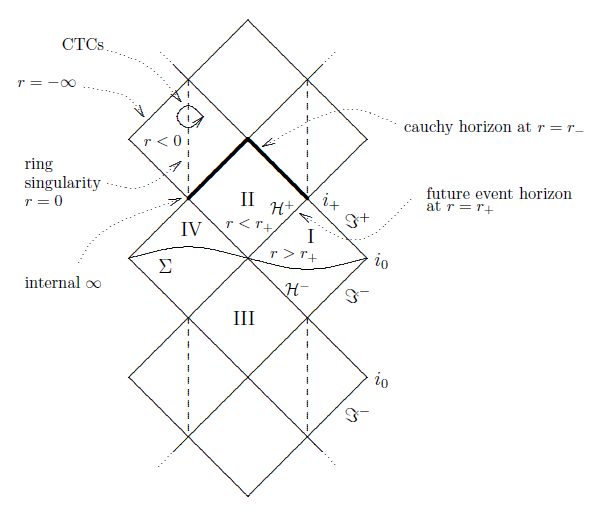
\includegraphics[scale=0.7]{immagini/kerr_causale_2.png}
    \caption{Struttura causale di Kerr $m^2 > a^2$ per $\theta = 0$. Il grafico può essere esteso in entrambe le direzioni (CTCs sta per \textit{closed timelike curves}).}
    \label{fig.kerr_causale_2}
\end{figure}
\subsubsection{$m^2 = a^2$}
Il buco nero di Kerr è estremo. Segue che $r_+=r_-= m$ e le gravità superficiali $\kappa_+ = \kappa_- = 0$; la temperatura di Hawking è pertanto nulla. L'orizzonte di Killing a $r = m$ è degenere ($\kappa =0)$ per il campo di Killing:
\begin{equation*}
    \xi = \partial_t + \Omega_H \partial_\phi \ \textrm{ con } \ \Omega_H = \frac{a}{2m}
\end{equation*}
Il diagramma di Penrose per questo caso è mostrato in fig. \ref{fig.kerr_causale_3}.
Si nota comunque che, nonostante possano esistere angoli $\theta$ per i quali possa avvenire il passaggio a $r<0$ attraverso $r=0$, questo fisicamente non si verifica in quanto nel collasso gravitazionale delle stelle non si verificano le condizioni per le quali questo \virgolette{ponte} sia attraversabile.
\begin{figure}
    \centering
    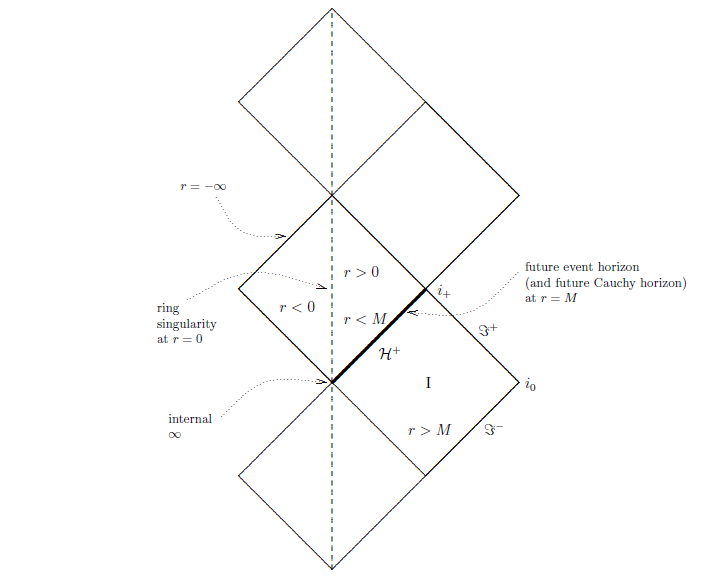
\includegraphics[scale=0.6]{immagini/kerr_causale_3.png}
    \caption{Struttura causale per Kerr estremale a $\theta =0$.}
    \label{fig.kerr_causale_3}
\end{figure}
\subsection{Ergosfera e processo di Penrose}
Calcoliamo:
\begin{equation*}
    <\partial_t, \partial_t > = g_{tt} = - \frac{\Delta - a^2\sin^2\theta}{\rho^2}= - \left(1 - \frac{2mr}{r^2+ a^2\cos^2\theta} \right)
\end{equation*}
Il vettore $\partial_t$ è di tipo tempo quando:
\begin{equation*}
    r^2 +a^2\cos^2\theta -2mr > 0
\end{equation*}
Nel caso $m^2 > a^2$ (interesse fisico) ciò avviene quando:
\begin{equation*}
    r > m + \sqrt{m^2 - a^2\cos^2\theta}
\end{equation*}
Il bordo di questa regione è un'ipersuperficie detta \textbf{ergosfera}: l'ergosfera è una superficie di tipo tempo che giace fuori dall'orizzonte $r=r_+$, ad eccezione di dove lo tocca a $\theta = 0, \pi$,  fig. \ref{fig.ergosfera}. In questi punti sull'asse di simmetria, diventa ipersuperficie nulla.
La regione interna dove $\partial_t$ può diventare di tipo spazio al di fuori dell'orizzonte degli eventi è detta \textbf{ergoregione}.


\begin{figure}
    \centering
    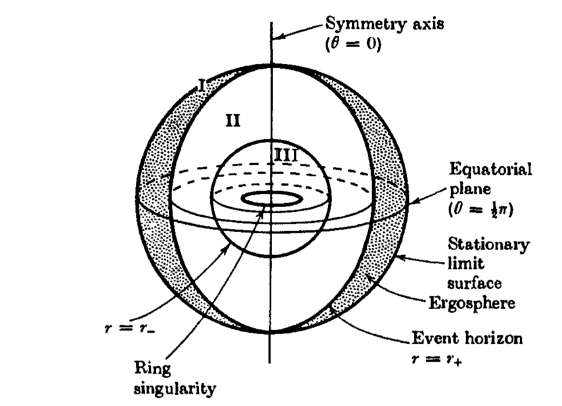
\includegraphics[scale=0.5]{immagini/ergosfera.png}
    \caption{Ergosfera del buco nero di Kerr per $m^2 > a^2$.}
    \label{fig.ergosfera}
\end{figure}

L'ergoregione permette dei processi fisici particolari: uno di questi è il \textbf{processo di Penrose}.
Consideriamo una particella che si avvicina lungo una geodetica al buco nero; chiamiamo $p$ il suo 4-momento (necessariamente tipo tempo). Per il vettore di Killing $k = \partial_t$ si identifica la costante del moto (costante lungo la geodetica):
\begin{equation*}
    E = - p\cdot k
\end{equation*}
con l'energia della particella. Se $k$ è di tipo tempo, allora $E>0$. Supponiamo che questa particella decada in due corpi, uno dei quali cade nel buco nero e uno scappa via. Per conservazione dell'energia si avrà:
\begin{equation*}
    E_2 = E - E_1
\end{equation*}
dove $E_1 = - p_1 \cdot k$ e $E_2 = - p_2 \cdot k$. Normalmente si avrà $E_1 > 0$ così che $E_2 < E$. Tuttavia se il decadimento avviene nell'ergoregione (è fuori da $r=r_+$ quindi può scappare), non vale necessariamente $E_1 > 0$, poiché $k = \partial_t$ potrebbe essere di tipo spazio. In quel caso avremmo per la particella che scappa ad infinito $E_2 > E$ ovvero l'estrazione di energia dal buco nero.

L'estrazione di energia dal buco nero ha però delle limitazioni. Per una particella che attraversa l'orizzonte $r= r_+ = m + \sqrt{m^2 - a^2}$ si ha:
\begin{equation*}
    - p_1 \cdot \xi \geq 0
\end{equation*}
dove $\xi = \partial_t + \Omega_H \partial_\phi$; quest'ultimo è un vettore nullo e future-directed sull'orizzonte (visto che è tipo tempo fuori dall'orizzonte), e $p_1$ è anch'esso future-directed e tipo tempo o nullo, a seconda che la particella sia massiva o meno. Pertanto, esplicitamente:
\begin{equation*}
    - < p_1, \partial_t > - \Omega_H < p_1, \partial_\phi > \geq 0 \iff  E_1 - \Omega_H L_1 \geq 0 
\end{equation*}
dove $L_1 = p_1 \cdot \partial_\phi$ è la componente del momento angolare della particella nella direzione di $\partial_\phi$. Otteniamo $L_1 \leq \frac{E_1}{\Omega_H}$, perciò:
\begin{equation*}
     \ E_1 < 0 \implies L_1 < 0 
\end{equation*}
Quindi in un processo di Penrose, il momento angolare del buco nero di Kerr viene ridotto. Dopo il processo, il buco nero acquisisce la massa $m + \delta m$ e momento angolare $J + \delta J$ con:
\begin{align*}
    \delta m = E_1 && \delta J = L_1
\end{align*}
e segue:
\begin{align*}
    \delta J \leq \frac{\delta m}{\Omega_H} &= \frac{\delta m}{\frac{a}{r_+^2 + a^2}} = 2m\left(m + \sqrt{m^2 - \frac{J^2}{m^2}}\right)\frac{m}{J}\delta m \\
    &= \frac{2m( m^2 + \sqrt{m^4 - J^2})}{J}\delta m
\end{align*}
ricordando che $J = ma$. Facendo qualche calcolo algebrico si può verificare facilmente che questa diseguaglianza è equivalente a:
\begin{equation*}
    \delta \left( m^2 + \sqrt{m^4 - J^2} \right) \geq 0
\end{equation*}
In un processo di Penrose la quantità tra parentesi deve aumentare. Questa ha un'interpretazione fisica che è strettamente legata ai principi termodinamici dei buchi neri, trattati con maggiore generalità in \S\ref{para.termo_bh}.

Calcoliamo l'area dell'orizzonte degli eventi del buco nero di Kerr. Per fare questo poniamoci sull'orizzonte, con $r= r_+$ ($\Delta = 0$) e $v = \textrm{cost.}$ nella metrica eq. \ref{eq.metrica_kerr_coord_kerr}, così quella indotta è:
\begin{equation*}
    ds^2 = \frac{(r^2_+ + a^2)^2}{r^2_+ + a^2\cos^2\theta}\sin^2\theta d\chi^2 + (r^2_+ + a^2\cos^2\theta)d\theta^2
\end{equation*}
da cui si ottiene la radice del determinante:
\begin{equation*}
    \sqrt{\sigma} = \left[ \frac{(r^2_+ + a^2)^2}{r^2_+ + a^2\cos^2\theta}\sin^2\theta(r^2_+ + a^2\cos^2\theta)  \right]^{1/2} = (r^2_+ + a^2)\sin\theta
\end{equation*}
Poiché siamo a raggio fissato, $d\chi = d\phi$ e pertanto ha gli stessi estremi di integrazione. L'area dell'orizzonte è quindi:
\begin{equation}
    A = \int \sqrt{\sigma}d\chi d\theta = \int_0^{2\pi}d\chi \int_0^\pi (r^2_+ + a^2)\sin\theta d\theta = 4\pi (r_+^2 + a^2)
    \label{eq.area_orizz_kerr}
\end{equation}
sostituendo $r^2_+ + a^2 = 2m(m+\sqrt{m^2 - a^2})$ e $J=ma$:
\begin{equation*}
    A = 8\pi\left( m^2 +\sqrt{m^4 - J^2}\right)
\end{equation*}
Quindi la condizione trovata prima corrisponde al secondo principio della termodinamica dei buchi neri:
\begin{equation*}
    \delta A \geq 0
\end{equation*}
E tale condizione limita la perdita di momento angolare ed estrazione di energia dal buco nero. L'area svolge il ruolo di entropia in un buco nero.

Definiamo la \textbf{massa irriducibile} del buco nero come:
\begin{equation*}
    m^2_{irr} = \frac{1}{2}\left( m^2 +\sqrt{m^4 - J^2}\right)
\end{equation*}
perciò la massa del buco nero dovrà essere tale che:
\begin{equation*}
    m^2 = m_{irr}^2 + \frac{J^2}{4m_{irr}^2} \geq m_{irr}^2
\end{equation*}
Se partiamo con un buco nero di massa $m_0$ e momento angolare $J_0$, si avrà la massa irriducibile iniziale $m_{0, irr} := m_{irr}(m_0,J_0)$. Dopo il processo di Penrose si avrà un momento angolare minore e quindi, per la relazione qui sopra:
\begin{equation*}
    m^2 \geq m^{2}_{irr} \geq m^2_{0, irr}
\end{equation*}
La condizione dell'area ci impone $\delta m^2_{irr} \geq 0$. Le quantità sono positive perciò facendone la radice otteniamo $-m \leq - m_{irr} \leq - m_{0,irr}$ ed infine:
\begin{equation*}
    m_0 - m \leq m_0 - m_{irr} \leq m_0 - m_{0, irr}
\end{equation*}
Il primo termine $m_0 - m$ equivale all'energia estratta dal processo che dovrà pertanto essere minore di $m_0 - m_{0, irr}$. Quest'ultima può essere interpretata come l'energia associata alla rotazione del buco nero, prima del processo. L'energia massima estraibile, corrispondente a $\delta m^2_{irr} = 0$, è proprio $m_0 - m_{0,irr}$ e successivamente a ciò il buco nero avrà la temperatura $T =0$.

\subsection{Forma canonica (ADM) della metrica di Kerr e temperatura di Hawking} 
La metrica di Kerr in 4-dim può essere scritta nella forma:
\begin{equation}
    ds^2 = - N^2 dt^2 + \sigma( d\phi - \omega dt)^2 + \frac{\rho^2}{\Delta}dr^2 + \rho^2 d\theta^2
    \label{eq.metrica_kerr_adm}
\end{equation}
dove sono stati definiti:
\begin{align*}
    N^2 &= \frac{\rho^2 \Delta}{\Sigma^2} \ \ \textrm{ (lapse function)} \\
    \Sigma^2 &= (r^2 +a^2)^2 - \Delta a^2 \sin^2\theta \\
    \sigma &= \frac{\Sigma^2}{\rho^2}\sin^2\theta \\
    \omega &= \frac{2mar}{\Sigma^2} \\
    \Delta &= r^2 -2mr + a^2
\end{align*}
Questa è la metrica di Kerr nella \textbf{forma canonica di ADM (Arnowitt, Deser, Misner)}.
La lapse function ha questo nome poiché, posta davanti a $dt^2$, fornisce informazioni su come scorre il tempo. In una generica dimensione, la forma canonica di ADM è del tipo:
\begin{equation*}
    ds^2 = -N^2dt^2 + n_{ij}(dx^i - N^idt)(dx^j - N^jdt)
\end{equation*}
Il formalismo di ADM è utilizzato per formulazioni hamiltoniane della relatività generale, in particolare nella quantizzazione canonica della gravità e in approcci numerici.

Come applicazione di questa metrica, possiamo vedere come calcolare più semplicemente la temperatura di Hawking, senza passare dal calcolo della gravità superficiale.
Eseguiamo una rotazione di Wick $t \rightarrow -i\tau$ per ottenere la metrica quasi euclidea:
\begin{equation*}
    ds_E^2 = N^2 d\tau^2 + \sigma(d\phi +i \omega d\tau)^2 + \frac{\rho^2}{\Delta}dr^2 + \rho^2 d\theta^2 
\end{equation*}
Sviluppiamo vicino all'orizzonte:
\begin{equation*}
    \Delta = \Delta(r_+) + \Delta'(r_+)(r-r_+) + \dots = 2(r_+ -m)(r-r_+) + \dots
\end{equation*}
\begin{equation*}
    N^2 = N^2(r_+) + \frac{\partial N^2}{\partial r}\Big|_{r_+}(r-r_+) + \dots =\frac{r_+^2 + a^2\cos^2\theta}{(r_+^2 + a^2)^2}2(r_+ - m)(r- r_+) + \dots
\end{equation*}
La metrica diventa:
\begin{align*}
    ds^2 \xrightarrow{r \rightarrow r_+} &\frac{r_+^2 + a^2\cos^2\theta}{(r_+^2 + a^2)^2}2(r_+ - m)(r- r_+) d\tau^2 + \frac{r_+^2 + a^2\cos^2\theta}{2(r_+ - m)(r- r_+)}dr^2 + \\
    & + \sigma_+(d\phi + i\omega_+ d\tau)^2 + \rho_+^2 d\theta^2
\end{align*}
Ponendo $R^2 = r- r_+$ otteniamo:
\begin{equation*}
    ds^2 \xrightarrow{r \rightarrow r_+} \frac{2(r_+^2 + a^2\cos^2\theta)}{r_+ - m}\left[ \frac{(r_+ -m)^2}{(r_+^2+ a^2)^2}R^2d\tau^2 + dR^2\right]
\end{equation*}
In questo modo la metrica è conforme a Minkowski se facciamo la corretta identificazione per $\tau$: otteniamo una singolarità conica a meno che:
\begin{equation*}
    \tau \sim \tau + 2\pi\frac{r_+^2 + a^2}{r_+ - m} \qquad \kappa = \frac{r_+-m}{r_+^2+a^2}
\end{equation*}
Così si ottiene la temperatura di Hawking per il buco nero di Kerr:
\begin{equation}
    T_H = \frac{r_+ - m}{2\pi(r_+^2 + a^2)} = \frac{r_+ - m}{4\pi m r_+}
    \label{eq.temp_hawking_kerr}
\end{equation}
Nel caso estremale $r_+ = m$ la temperatura è nulla.
\subsection{Trascinamento dei sistemi di riferimento inerziali}
Un altro fenomeno associato all'ergoregione è il cosiddetto \textit{frame dragging} o trascinamento del sistema di riferimento: i corpi nell'ergoregione non possono stare a coordinata $\phi = \textrm{cost.}$, ma sono costretti a ruotare nella stessa direzione del buco nero, altrimenti dovrebbero muoversi a velocità superluminari.
Questo effetto, come vedremo fra poco, è legato nuovamente alla natura della componente $g_{tt}$ che in questa regione cambia di segno e diventa tipo spazio (dunque i corpi non possono seguire in maniera causale una traiettoria statica con $r, \theta, \phi = \cost$).

Consideriamo quindi una linea di mondo di tipo tempo con $u$ il suo vettore tangente: $u^2 < 0$.
Esplicitamente, usando la forma di ADM, eq. \ref{eq.metrica_kerr_adm}:
\begin{equation*}
    g_{tt}u^tu^t + g_{\phi\phi}u^\phi u^\phi + g_{\theta\theta}u^\theta u^\theta + g_{rr}u^r u^r + 2g_{t\phi}u^t u^\phi < 0
\end{equation*}
Si ha che i termini in $g_{\phi\phi}, g_{\theta\theta}, g_{rr}$ sono positivi (tipo spazio) e anche $g_{tt} > 0$ poiché nell'ergoregione. Perciò si deve avere $g_{t\phi}u^t u^\phi < 0$ e poiché $g_{t\phi} = - \omega \sigma < 0$ dalla definizione della metrica eq. \ref{eq.metrica_kerr_adm}, allora il segno di $u^t u^\phi$ dovrà essere positivo. 

Mostriamo che $u^t > 0$.  Consideriamo $\xi = \partial_t + \omega \partial_\phi$, $< \xi, \xi > = -N^2 < 0$; $\xi$ è di tipo tempo al di fuori dell'orizzonte, mentre è nullo sull'orizzonte di cui è generatore. Inoltre è future-directed in quanto all'infinito $\omega \sim r^{-3} \rightarrow 0$ e rimane $\partial_t $ che è future-directed.
Poiché anche $u$ è timelike, future-directed, si ha che $< u, \xi > < 0$. Nel dettaglio:
\begin{equation*}
    <u, \partial_t > + \omega < u, \partial_\phi > \ < 0
\end{equation*}
\begin{equation*}
    < u^t \partial_t + u^\phi \partial_\phi + u^\theta \partial_\theta + u^r\partial_r, \partial_t > + \omega < u^t \partial_t + u^\phi \partial_\phi + u^\theta \partial_\theta + u^r\partial_r, \partial_\phi > \ < 0 \\
\end{equation*}
Poiché non vi sono termini in $g_{\theta t}, g_{rt}, g_{\theta\phi}, g_{r\phi}$ rimangono:
\begin{equation*}
    u^t g_{tt} + u^\phi g_{\phi t} + \omega( u^t g_{\phi t} + u^\phi g_{\phi\phi}) <0
\end{equation*}
\begin{equation*}
    u^t( -N^2 + \omega^2\sigma) +u^\phi(-\omega \sigma) +\omega( u^t(-\omega\sigma) + u^\phi\sigma) <  0
\end{equation*}
Semplificando rimane $-N^2 u^t < 0$ e quindi $u^t > 0$.

Dunque si ha che $u^\phi > 0$ ovvero, rispetto un parametro affine $\tau$:
\begin{equation*}
    u^\phi = \frac{d\phi}{d\tau} > 0
\end{equation*}
Quindi come detto la coordinata di rotazione intorno all'asse non può rimanere costante in questa regione e il corpo è costretto a rimanere in rotazione col buco nero. Può tuttavia ancora fuggire da esso, poiché è fuori dall'orizzonte degli eventi.

\subsection{Generalizzazioni di Myers-Perry}
Vediamo ora delle generalizzazioni alla soluzione di Kerr per dimensioni maggiori. In generale per $R_{\mu\nu} =0 $ e $d \geq 4$ il gruppo di isometrie è $SO(d-1)$ dal quale ci sono $\lfloor\frac{d-1}{2}\rfloor$ Casimir distinti; questi sono i parametri indipendenti di un generale tensore momento angolare. Un buco nero rotante generico avrà quindi $n+1$ parametri caratterizzanti: la massa $m$ e gli $n$ momenti angolari commutanti.
Il motivo per cui soluzioni a dimensione maggiore sono interessanti sono proprio queste nuove direzioni di rotazione possibili: buchi neri in più dimensioni assumono forme particolari e infatti si parla di \textit{black ring}, \textit{black saturn} \dots. Una review di questo tipo di soluzioni è stata fatta da R. Myers stesso in \cite{myers}.

Consideriamo quindi in $d \geq 4$, per semplicità, la soluzione \virgolette{single spinning} nella quale una sola componente rotante è presente. La metrica è:
\begin{align}
    ds^2 &= -dt^2 + \frac{\mu}{r^{d-5}\rho^2}(dt + a\sin^2\theta d\phi)^2 + \frac{\rho^2}{\Delta}dr^2 + \rho^2d\theta^2 + \nonumber \\
    &(r^2 + a^2)\sin^2\theta d\phi^2 +r^2\cos^2\theta d\Omega^2_{d-4}
    \label{eq.metrica_myers_perry_singlespinning}
\end{align}
con $\rho^2 = r^2 +a^2\cos^2\theta$, $\Delta = r^2 + a^2 - \frac{\mu}{r^{d-5}}$ e $\mu$ un parametro di massa. Questa soluzione ha orizzonte nella soluzione più grande di $\Delta = 0$:
\begin{itemize}
    \item $d=5$ l'orizzonte esiste solo per $\mu > a^2$
    \item $d > 5$ c'è sempre orizzonte, senza limiti sul momento angolare
\end{itemize}

Anche in questo caso, come nell'estremale i Reissner-Nordstr\"om, si può investigare la \virgolette{competizione} tra l'attrazione gravitazionale e la repulsione centrifuga considerando:
\begin{equation*}
    \frac{\Delta}{r^2} -1 = - \frac{\mu}{r^{d-3}}+ \frac{a^2}{r^2}
\end{equation*}
Il primo termine a destra corrisponde al potenziale gravitazionale newtoniano generalizzato, mentre il secondo termine è quello centrifugo, con dipendenza $r^{-2}$. Viene mantenuta questa dipendenza poiché, nonostante siamo in maggiori dimensioni, la rotazione avviene sempre in un piano e quindi il termine centrifugo rimane invariato. Si deduce che per:
\begin{itemize}
    \item $d=4$ vince il potenziale gravitazionale e c'è limite a Kerr ovvero non si può avere un momento angolare grande arbitrariamente (come già osservato nel caso non causale $m^2 < a^2$).
    \item $d >5$ vince il potenziale centrifugo e non c'è limite alla rotazione.
\end{itemize}
Come conseguenza della rotazione non limitata del caso a $d>5$, c'è la possibilità di assumere valori $a$ molto grandi e in questo caso si parla di \textit{ultra spinning Myers-Perry}: per valori sufficientemente elevati di $a$ si ha la situazione di uno \textit{spinning pancake}.

\subsection{Near Horizon limit del Kerr estremo}
Torniamo al Kerr in 4-dim per considerare nuovamente il caso estremo. Con Reissner-Nordstr\"om si era visto che la geometria vicino all'orizzonte era del tipo $AdS_2 \times S^2$. Vediamo cosa succede nel Kerr con $m=a$, $r_+ =r_-= m$ oltre a determinare $T_H = 0$ e $\omega_H = \frac{1}{2m}$. La metrica in coordinate di Boyer-Lindquist è:
\begin{equation*}
    ds^2 = - \frac{\Delta}{\rho^2}\left(d\hat{t}^2 -a^2 \sin^2\theta d\hat{\phi}\right)^2 + \frac{\sin^2\theta}{\rho^2}\left((\hat{r}^2 + a^2)d\hat{\phi} - ad\hat{t} \right)^2 + \rho^2 d\theta^2 + \frac{\rho^2}{\Delta}d\hat{r}^2
\end{equation*}
dove $\Delta = (\hat{r} - a)^2$. Per ottenere il limite vicino all'orizzonte si introduce un parametro di scaling $\lambda\rightarrow 0$ nelle nuove coordinate:
\begin{align*}
    r &= \frac{\hat{r}-m}{\lambda m} \\
    t &= \frac{\lambda \hat{t}}{2m} \\
    \phi &= \hat{\phi} - \frac{\hat{t}}{2m}
\end{align*}
che vengono mantenute fisse mentre si manda $\lambda$ a zero. In questo limite la metrica diventa:
\begin{equation*}
    ds^2 = 2\Omega^2 J\left[ \frac{dr^2}{r^2}  - r^2dt^2 + d\theta^2 + \Lambda^2(d\phi +rdt)^2\right]
\end{equation*}
con $\Omega^2 = \frac{1}{2}(1+\cos^2\theta)$ e $\Lambda =\frac{2\sin\theta}{1+\cos^2\theta}$.
Si può riconoscere dai  primi due termini $AdS_2$, tuttavia Kerr non risulta spazio prodotto poiché $\Omega^2(\theta)$. Se consideriamo però $\theta = \textrm{cost.} =: \theta_0$ e fissato tale che $\Lambda(\theta_0) = 1$, allora si ottiene $AdS_3$.
Il gruppo di isometrie è $SL(2, \mathbb R) \times U(1)$; il primo segue come gruppo di isometrie di $AdS_2$, mentre il secondo dalle traslazioni di $\phi$. In questa maniera il near horizon di Kerr è molto simile a quello di Reissner-Nordstr\"om.